\section{Anleihen und grundlegende Beispiele für Derivate}

Hier betrachten wir immer nur ein Basisgut $S_t = S_t^1$.

\begin{enumerate}[leftmargin=*, label=(\alph*)]
	\item \begriff{Anleihe} [bond] (genauer: Null-Kupon-Anleihe [zero-coupon bond]) --- siehe \cref{fig: zahlungsstromAnleihe}
	
	Der Emittent (Herausgeber) einer Anleihe mit Endfälligkeit [maturity] $T$ garantiert dem Käufer zum Zeitpunkt $T$ den Betrag $N$ (EUR/USD/...) zu zahlen.
	Typische Emittenten sind z.B. Staaten [government bond] oder Unternehmen (als Alternative zur Kreditaufnahme).
	Nach Emission werden Anleihen auf dem Sekundärmarkt weiterverkauft, d.h. liquide gehandelte Wertpapiere. 
	
	\begin{tabular}{ll}
		Preis bei Emission: & $B(0,T)$ \\
		Preis bei Weiterverkauf zum Zeitpunkt $t \le T$: & $B(t,T)$ \\
	\end{tabular}
	
	Es ist $B(T,T) = N$ und wir normieren stets $N=1 \follows B(T,T)=1$.
	
	Anleihen von West-/ Nord-/ Mitteleuropäischen Staaten und den USA sowie Kanada werden als risikolos betrachtet (sichere Zahlung). Sonst: Kreditrisiko
	
	Risikofreie Anleihen können als Numeraire $S_t^0 = B(t,T)$ genutzt werden.
	
	\begin{figure}
		\centering
		\begin{minipage}[t]{\dimexpr0.45\linewidth-\fboxrule-\fboxsep}
			\centering
			%TODO BILD (1)
			\includegraphics[width=.9\textwidth]{example-image}
			\caption{Zahlungsstrom einer Anleihe}
			\label{fig: zahlungsstromAnleihe}
		\end{minipage}
		\begin{minipage}[t]{\dimexpr0.5\linewidth-\fboxrule-\fboxsep}
			\centering
			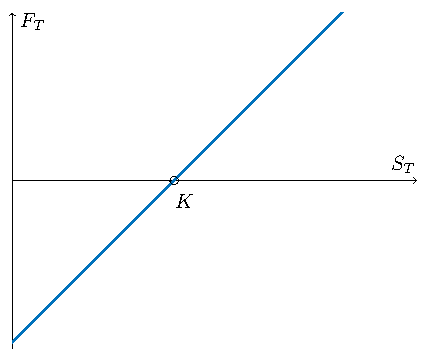
\includegraphics[width=.9\textwidth]{img/terminvertrag}
			\caption{Auszahlungsprofil eines Terminvertrags}
			\label{fig: terminvertrag}
		\end{minipage}
	\end{figure}
	
	\item \begriff{Terminvertrag} [forward contract]
	
	Aus Käufersicht besteht ein Terminvertrag aus der Vereinbarung zu bestimmtem zukünftigen Zeitpunkt $T$ eine Einheit des Basisguts $S$ zum Preis $K$ zu kaufen (Kaufverpflichtung). Beliebt ist dieser bei Rohstoffen und Elektrizität. Ist der Preis zum Zeitpunkt $t$ gegeben durch $F_t$, so lässt sich das Auszahlungsprofil (siehe \cref{fig: terminvertrag}) schreiben als 
	\begin{equation*}
		F_T = S_T - K .
	\end{equation*}
	
	
	\item \begriff{(Europäische) Put- bzw. Call-Option}
	
	\textit{Recht} zu einem zukünftigen Zeitpunkt $T$ eine Einheit des Basisguts $S$ zum Preis $K$ zu verkaufen (Put) bzw. zu kaufen (Call)
	$\leadsto$ keine Kaufverpflichtung!
	% Vergleich zum Terminvertrag: keine Pflicht
	
	\begin{center}
		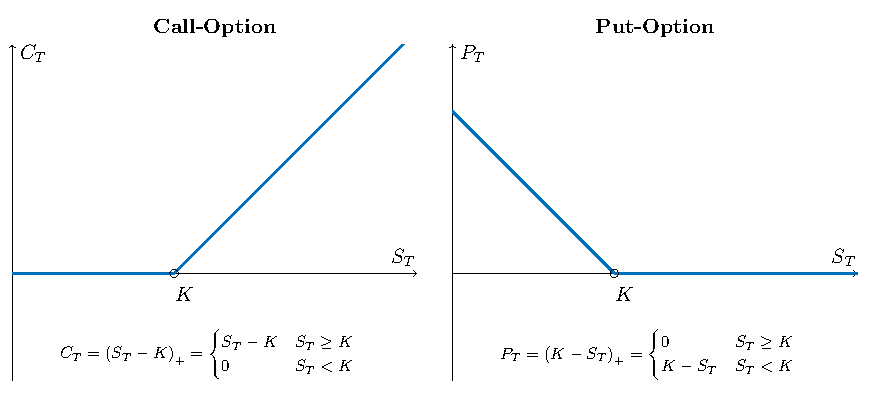
\includegraphics[width=\linewidth]{./img/call-put-auszahlungsprofil}
		\captionof{figure}{Auszahlungsprofile von Call- und Put-Optionen}
	\end{center}


	\item \begriff{Amerikanische Put- bzw. Call-Option}
	
	wie Put/Call, aber mit Ausübung zu beliebigem Zeitpunkt $\tau \in [0,T]$.
	
	\begin{tabular}{ll}
		Preis zum Zeitpunkt $t$: & $P_t^{AM}$, $C_t^{AM}$ \\
		Auszahlungsprofil zum Zeitpunkt $\tau$: & $\brackets{S_\tau - K}_+$, $\brackets{K - S_\tau}_+$
	\end{tabular}
	
	Der Zeitpunkt $\tau$ muss im Allgemeinen als Lösung eines stochastischen Optimierungsproblems bestimmt werden (Optimales-Stopp-Problem).
\end{enumerate}